\subsection{送信波形の計測}
ラインフォーカス探触子先端部を供試体に接触させず、自由に振動させたときの挙動を調べた。
振動波形の取得にはLDVを用い、探触子の駆動は、前節に示した条件で行った。
その結果として得られた、探触子先端部の振動波形を図\ref{fig:fig5}に示す。
この図の(a)は振動速度の時刻歴を、(b)はその周波数スペクトルを示している。
時刻歴波形からは、シュー内部を超音波が伝播することに伴う時間遅れが約11$\mu$secであることが
読み取れる。また振幅はpeak-to-peakでおよそ0.4V程度となっている。
別途行った、2.25MHZ、直径22.5mmの垂直接触型トランスデューサに比べ、約20倍程度大きな振幅値である。
これにより、圧電素子からの縦波がシュー先端部に集束し、強い超音波が発生していることが分かる。
周波数スペクトルからは、周波数帯域の上限が約3MHz、主たる周波数成分は1〜2MHに
あることが示されている。なお、シュー先端部で反射された波が、再度先端部に集束する
ことも確認しているが、その波形成分は30$\mu$sec付近にあり、時間軸上で完全に分離できるため、
計測の障害にはならない。
%--------------------
\begin{figure}[h]
	\begin{center}
	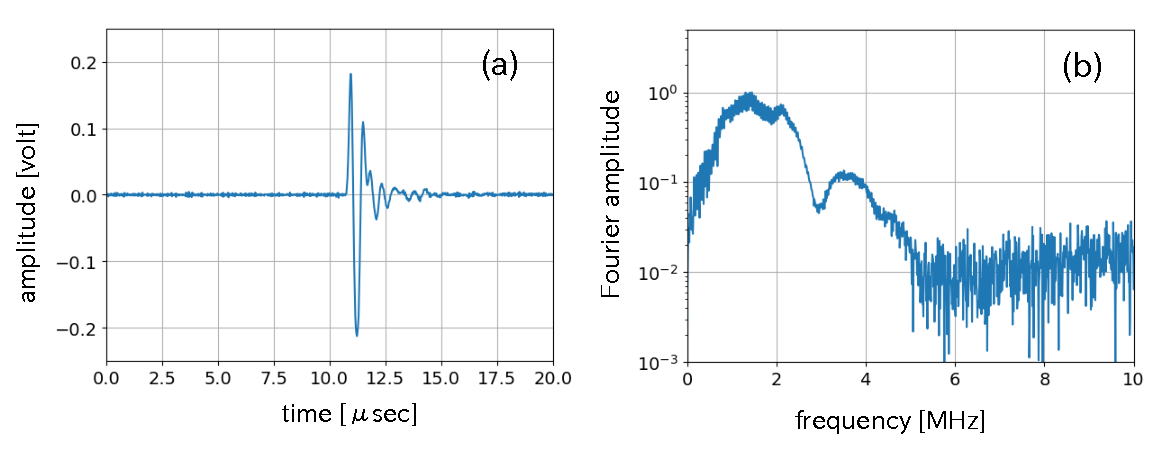
\includegraphics[width=0.9\linewidth]{Figs/fig5.eps} 
	\end{center}
	\caption{
		レーザードップラー振動計で計測した,ラインフォーカス探触子シュー先端部の振動速度波形.
	} 
	\label{fig:fig5}
\end{figure}
%--------------------
\subsection{透過波波形}
花崗岩コア供試体を用いて計測した透過波の計測結果を図\ref{fig:fig5_2}と\ref{fig:fig5_3}に示す。
これらの図には、それぞれ、入射方向の異なる6つの走時プロットが示されている。
各々の走時プロットの横軸は時間$t$($\mu$sec)を、縦軸は計測位置の$y$座標(mm)を表し,
$(t,y)$で観測された波形の振幅をカラー表示したものである。
なお、波形振幅は、最大値で無次元化している。
いずれの入射方向でも、19$\mu$sec前後に大きな振幅を持つ位相の揃った表面波が到達し、その後、
多重散乱に起因するコーダ波が、少なくとも20$\mu$sec程度継続して観測されている。
位相の揃った初動成分の振幅は場所によって大きな変動があり、波形も位置や入射方向によって異なることが分かる。
このことから、個々の観測波形のピーク位置や到達時間から、伝播速度を正確に求めることは困難と言える。
そこで以下では、群遅延から求めた群速度と、
相互相関関数によって評価した遅延時間から求めた音速を用いて、
供試体の音響異方性について調べる。
なお、
%--------------------
\begin{figure}[h]
	\begin{center}
	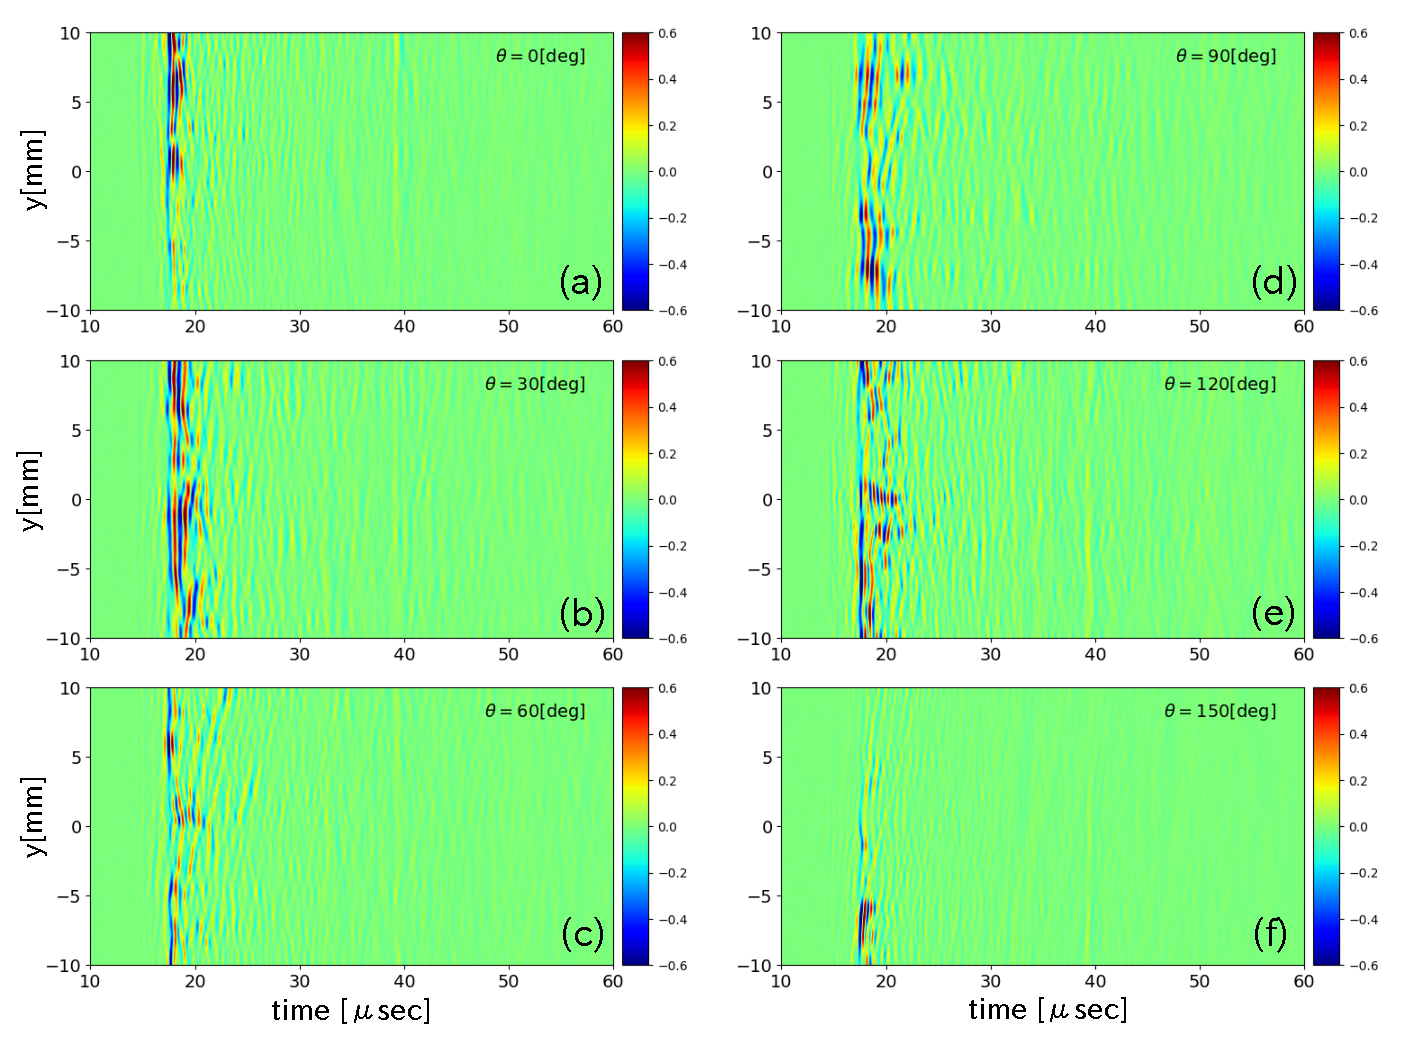
\includegraphics[width=1.0\linewidth]{Figs/fig5_2.eps} 
	\end{center}
	\caption{
		透過波波形の走時プロット(入射方向$\theta=0\sim 150^{\circ}$)
	} 
	\label{fig:fig5_2}が
\end{figure}
%--------------------
\begin{figure}[h]
	\begin{center}
	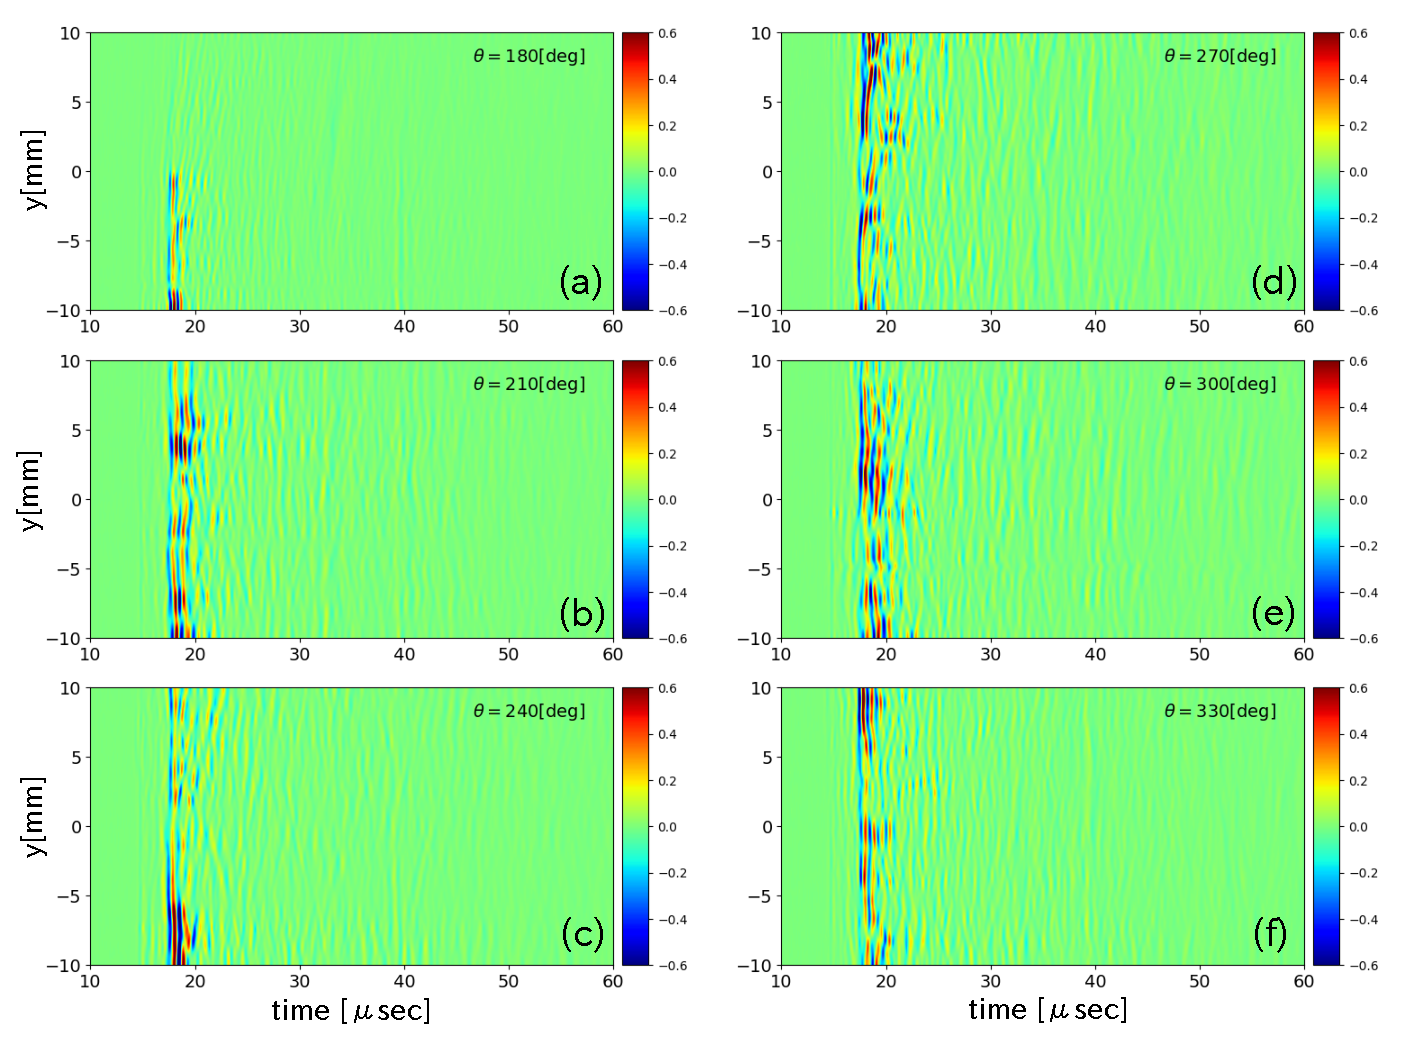
\includegraphics[width=1.0\linewidth]{Figs/fig5_3.eps} 
	\end{center}
	\caption{
		透過波波形の走時プロット(入射方向$\theta=180\sim 330^{\circ}$)
	} 
	\label{fig:fig5_3}
\end{figure}
\subsection{伝播速度の評価}
位相の揃った初動成分を対象として伝播速度の評価を行う。
そのため、時間波形上で窓関数を作用させて初動部分を取り出す。
その際、ここではButterworth関数を用いる。
\begin{equation}
	W(t;t_{1/2},m)=
	\left\{
		1+\left(\frac{t}{t_{1/2}}\right)^m
	\right\}^{-1}
\end{equation}
\begin{equation}
	a(y,t)=a_{mes}(y,t)W(t-t_b;t_{1/2},m)
\end{equation}
ただし、$t_b=18.2$[$\mu$sec], $t_{1/2}=2$[$\mu$sec]で$m=6$.
個々の波形は伝播経路やその周辺の鉱物流の影響を受けて変動する。
何らかの平均値を求める必要がある。
空間的な平均波形を
\begin{equation}
	\left< a\right>(t)=
	\frac{1}{\left| {\cal R}\right|}\int_{\cal R}a(y,t)dy
	\label{eqn:def_mean_wv}
\end{equation}
で定義し、この平均波形から速度を求める。
同時に、個々の計測波形$a(y,t)$から求めた速度の平均値の入射方向依存性を見る。
速度は、群遅延から評価した速度を$c_g$,相互相関から評価した速度を$c_{cor}$と表す。
また、平均波形から評価した速度を$\bar c$, 速度の平均値を$\left< c_{cor}\right>$と表す。
波形$a(t)$のフーリエ変換を
\begin{equation}
	A(\omega)=\int a(t)e^{-i\omega t}dt=\left| A(\omega) \right|e^{i\phi}
	\label{eqn:def_FFT}
\end{equation}
\begin{equation}
	t_g=-\frac{d\phi}{d\omega}
	\label{eqn:}
\end{equation}
\begin{equation}
	c_g=\frac{L}{t_g-t_g^{ref}}
	\label{eqn:def_cg}
\end{equation}
$\bar{c}_g$は、式(\ref{eqn:def_FFT})において$a(t)=<a(y,t)>$としたときに式(\ref{eqn:def_tg})
と式(\ref{eqn:def_cg})から得られる群速度を意味する.
%--------------------
\begin{figure}[h]
	\begin{center}
	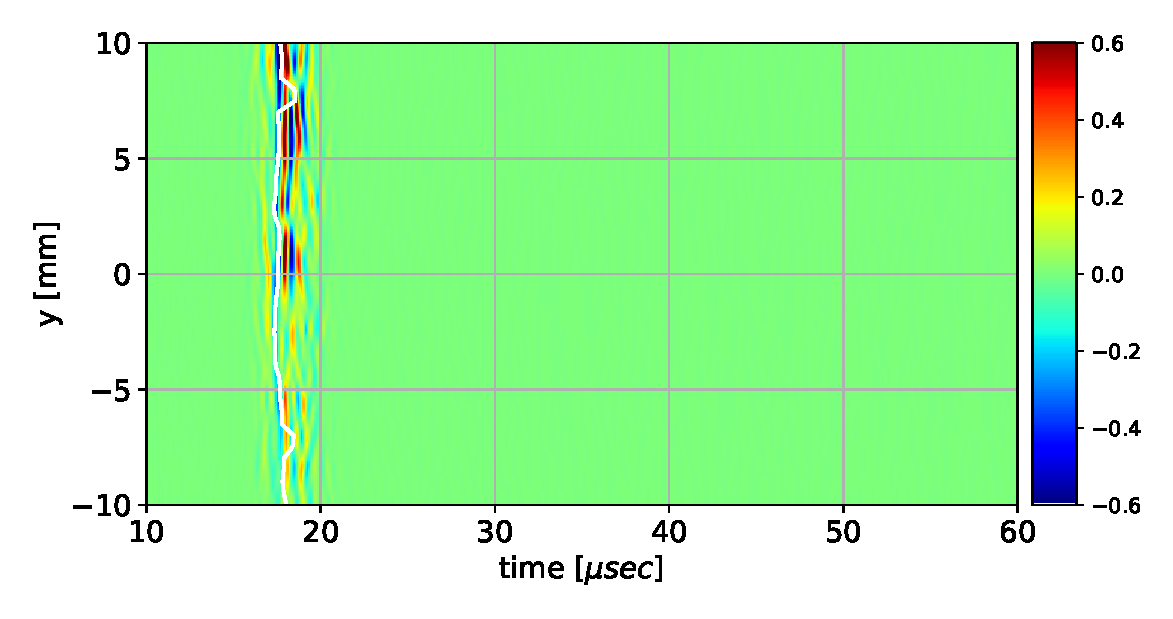
\includegraphics[width=0.7\linewidth]{Figs/fig6.eps} 
	\end{center}
	\caption{
		計測波形の走時プロット(入方向$\theta=0^{\circ}$)
	} 
	\label{fig:fig6}
\end{figure}
%--------------------
\begin{figure}[h]
	\begin{center}
	\includegraphics[width=0.7\linewidth]{Figs/fig7.eps} 
	\end{center}
	\caption{
		計測波形の周波数スペクトログラム(入方向$\theta=0^{\circ}$)
	} 
	\label{fig:fig7}
\end{figure}
%--------------------
\begin{figure}[h]
	\begin{center}
	\includegraphics[width=0.6\linewidth]{Figs/fig8.eps} 
	\end{center}
	\caption{
		平均波形の時刻歴(入射方向$\theta=0^{\circ}$の場合).
	} 
	\label{fig:fig8}
\end{figure}
%--------------------
\begin{figure}[h]
	\begin{center}
	\includegraphics[width=0.6\linewidth]{Figs/fig9.eps} 
	\end{center}
	\caption{
		平均波形の周波数スペクトル(入射方向$\theta=0^{\circ}の場合$).
	} 
	\label{fig:fig9}
\end{figure}
%--------------------
\begin{figure}[h]
	\begin{center}
	\includegraphics[width=0.7\linewidth]{Figs/fig10.eps} 
	\end{center}
	\caption{
		平均波形の位相スペクトル(入射方向$\theta=0^{\circ}$の場合).
	} 
	\label{fig:fig10}
\end{figure}
%--------------------
